\subsection{Simulated Annealing}

Simulated annealing is a stochastic algorithm that attempts to find the global optimum of an objective function $f(x)$. The method is inspired by statistical physics, in particular the Boltzmann distribution that specifies the probability of being in a particular state $x$:
\begin{equation}
    p(x) \propto \exp\{-f(x)/T\}
\end{equation}
where $f(x)$ is the energy of the system and $T$ is the temperature. As the temperature approaches zero, the system spends more and more time in its minimum energy (most probable) state. As the temperature decreases, the largest peaks become larger and the smallest peaks dissappear. By cooling slowly enough, it is possible to track the largest peak and therefore find the global optimum.\\

Simulated annealing is closely related to the Metropolis-Hastings algorithm for generating samples from a probability distribution. At each step of the algorithm, we sample a new state according to a proposal distribution $x^{\prime} \sim q(\dot|x_k)$, such as a random walk proposal:
\begin{equation}
    x^{\prime} = x_k + \epsilon_k, ~~~ \mathrm{where}~ \epsilon_k \sim N(0,\Sigma)
\end{equation}
Having proposed a new state, we compute $\alpha$ as in Algorithm \ref{alg:sim_annealing}.
\begin{algorithm}
\caption{Simulated Annealing}
\label{alg:sim_annealing}
\begin{algorithmic}[1]
\STATE $\alpha = \exp\{(f(x)-f(x^{\prime}))/T\}$
\STATE $r = \min(1,\alpha)$
\STATE $u \sim \mathrm{Unif}(0,1)$
\STATE if $u < r$ 
\STATE ~~~ $x_{k+1} = x^{\prime}$
\STATE else
\STATE ~~~ $x_{k+1} = x_k$
\STATE end if  
\end{algorithmic}
\end{algorithm}
Thus, if a new state has lower energy (higher probability), we will definitely accept it but if it has higher energy (lower probability), we might still accept it depending on the temperature. Therefore, the algorithm allows downhill moves in probability space but less frequently as the temperature drops. In practice it is common to use an exponential cooling schedule: $T_k = T_0 C^{k}$, where $T_0 \sim 1$ is the initial temperature and $C \sim 0.8$ is the cooling rate. Cooling too quickly can result in getting stuck in local optima, while cooling too slowly wastes time. The optimum cooling schedule is difficult to determine.    

\begin{figure}[tbhp]
    \centering
    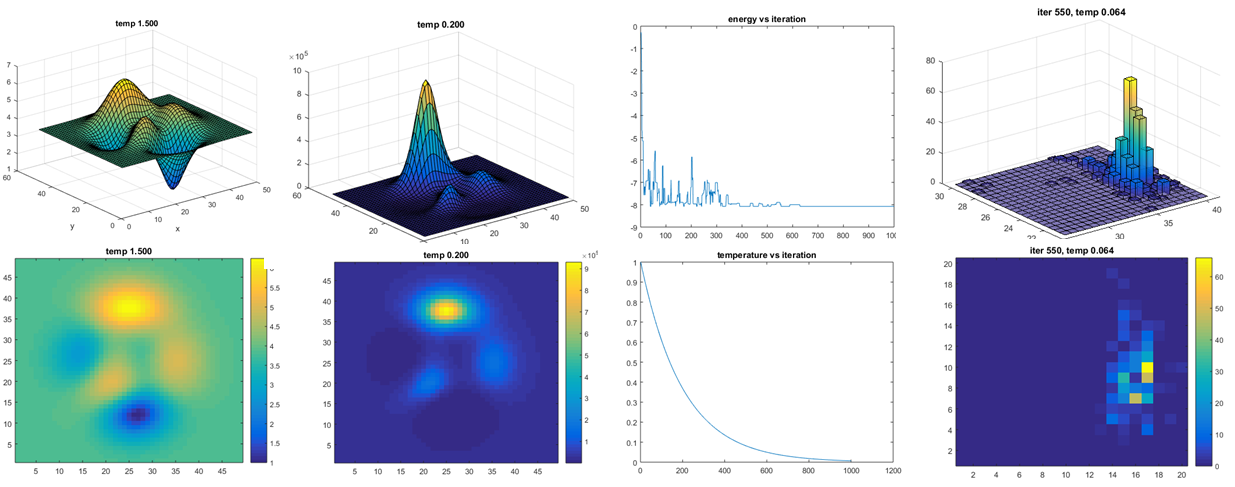
\includegraphics[width=0.9\textwidth, trim={10 10 10 10}]{figures/sim_annealing_merged.png}
    \caption{Simulated Annealing}
    \label{fig:sim_annealing_merged}
\end{figure}

Figure \ref{fig:sim_annealing_merged} shows the objective $f(x)$ at two different temperatures (left). The function appears more peaky when the temperature is lower. We can also see that the method stochastically reduces the energy over time for the given cooling schedule (middle). Finally a histogram of samples shows that most samples are concentrated near the global maximum (right).


\subsection{Bayesian Optimization}

Machine learning algorithms frequenty require careful tuning of hyperparameters. Often exhaustive and computationally expensive methods such as grid search cross validation are used to find model parameters that optimize a suitable performance objective. An alternative to grid search is randomized parameter optimization that samples parameter settings from a distribution over possible parameter values. This has two main benefits over the exhaustive search: the number of iterations can be chosen independent of the number of parameters and adding parameters that do not influence performance does not decrease efficiency. Rather than exploring the parameter space randomly (according to a chosen distribution), it would be great to adapt an active learning approach that selects parameter values in a way that reduces uncertainty and provides a balance between exploration and exploitation. Bayesian optimization provides an automated Bayesian framework by utilizing Gaussian Processes (GPs) to model algorithm's generalization performance \cite{snoek2012}.\\

Bayesian optimization assumes that a suitable performance function was sampled from a Gaussian Process and maintains a posterior distribution for this function as observations are made: $f(x)\sim \mathrm{GP}(m(x),\kappa(x,x^{\prime}))$. To choose which hyperparameters to explore next, one can optimize the Expected Improvement (EI) over the current best result or the Gaussian process Upper Confidence Bound (UCB). EI and UCB have been shown to be efficient in the number of function evaluations required to find the global optimum of multi-modal black-box functions. Bayesian optimization uses all of the information available from previous evaluations of the objective function as opposed to relying on local gradient and Hessian approximations. This results in an automated procedure that can find an optimum of non-convex functions with relatively few evaluations, at the cost of performing more computation to determine the next point to try. This is particularly useful when evaluations are expensive to perform such as in selecting hyperparameters for deep neural networks.\\

To determine what point should be evaluated next, we need to choose and acquisition function which is used to construct a utility function from the GP posterior. In general, the acquisition function depends on previous observations as well as GP hyperparameters that we denote as $a(x;\{x_n,y_n\},\theta)$, then $x_{next} = \arg \max_x a(x)$. Let $\mu(x;\{x_n,y_n\},\theta)$ be the predictive GP mean function, $\sigma^{2}(x;\{x_n,y_n\},\theta)$ be the predictive GP variance function and $\Phi(x)$ be the cumulative distribution function of the standard normal. Then we can define the following acquisition functions.\\

\textit{Probability of Improvement}. This strategy maximizes the probability of improving over the best current value. This can be computed as follows:
\begin{equation}
    a_{PI}(x;\{x_n,y_n\},\theta) = \Phi(\gamma(x)), ~~~~ \gamma(x) = \frac{f(x_{best}) - \mu(x; \{x_n,y_n\},\theta)}{\sigma(x;\{x_n,y_n\},\theta)}
\end{equation}

\textit{Expected Improvement}. Alternatively, one could choose to maximize the expected improvement (EI) over the current best. 
\begin{equation}
    a_{EI}(x;\{x_n,y_n\},\theta) = \sigma(x;\{x_n,y_n\},\theta)(\gamma(x)\Phi(\gamma(x))+N(\gamma(x);0,1))
\end{equation}

\textit{Upper Confidence Bound}. UCB is the idea of exploiting upper confidence bounds to construct acquisition functions that minimize regret over the course of their optimization. These acquisition functions have the following form:
\begin{equation}
    a_{UCB}(x;\{x_n,y_n\},\theta) = \mu(x;\{x_n,y_n\},\theta) - \kappa \sigma(x;\{x_n,y_n\},\theta)
\end{equation}
where $\kappa$ is a tunable acquisition parameter to balance exploration and exploitation. The optima of acquisition functions are located where the uncertainty in GP posterior is large (exploration) and/or where the GP prediction is high (exploitation). Since acquisition functions have analytical forms that are simple to evaluate, they are easier to optimize then the original objective function.\\

An important practical consideration for Bayesian optimization is an appropriate choice of GP kernel and its associated hyperparameters. Squared exponential kernel is often a default choice for Gaussian process regression. However, sample functions with this kernel are too smooth for practical optimization problems. Instead the following ARD Matern $5/2$ kernel is proposed:
\begin{eqnarray}
    K_{M52}(x,x^{\prime}) &=& \theta_0\bigg(1+\sqrt{5r^2(x,x^{\prime})}+\frac{5}{3}r^2(x,x^{\prime}) \bigg)\exp \{-\sqrt{5r^2(x,x^{\prime})}\}\\
    r^2(x,x^{\prime}) &=& \sum_{d=1}^{D}(x_d - x^{\prime}_d)^{2}/\theta_{d}^{2}
\end{eqnarray}
This kernel results in sample functions that are twice-differentiable without requiring the smoothness of the squared exponential kernel. The associated kernel hyperparameters are $D$ length scales $\theta_{1:D}$, the covariance amplitude $\theta_0$, the observation noise $\nu$ and a constant mean $m$. An additional assumption made by GP regression is that the underlying process is stationary, i.e. we can re-write the kernel $k(x,x^{\prime})$ as a function of $x-x^{\prime}$. Intuitively, a function whose length scale does not change throughout the input space will be modelled well by a GP with a stationary kernel.\\ 

Bayesian Optimization algorithm is summarized in Algorithm \ref{alg:bayes_opt}.
\begin{algorithm}
\caption{Bayesian Optimization}
\label{alg:bayes_opt}
\begin{algorithmic}[1]
\STATE \textbf{for} $n=1,2,...$ \textbf{do}
\STATE ~~~ select new $x_{n+1}$ by optimizing acquisition function $\alpha$\\
~~~ ~~~ $x_{n+1} = \arg \max_x \alpha(x;D_n,\theta)$
\STATE ~~~ query objective function to obtain $y_{n+1} = f(x_{n+1})$
\STATE ~~~ augment data $D_{n+1} = \{D_n,(x_{n+1},y_{n+1})\}$
\STATE ~~~ update GP posterior and acquisition function 
\STATE \textbf{end for}  
\end{algorithmic}
\end{algorithm}


\begin{figure}[tbhp]
    \centering
    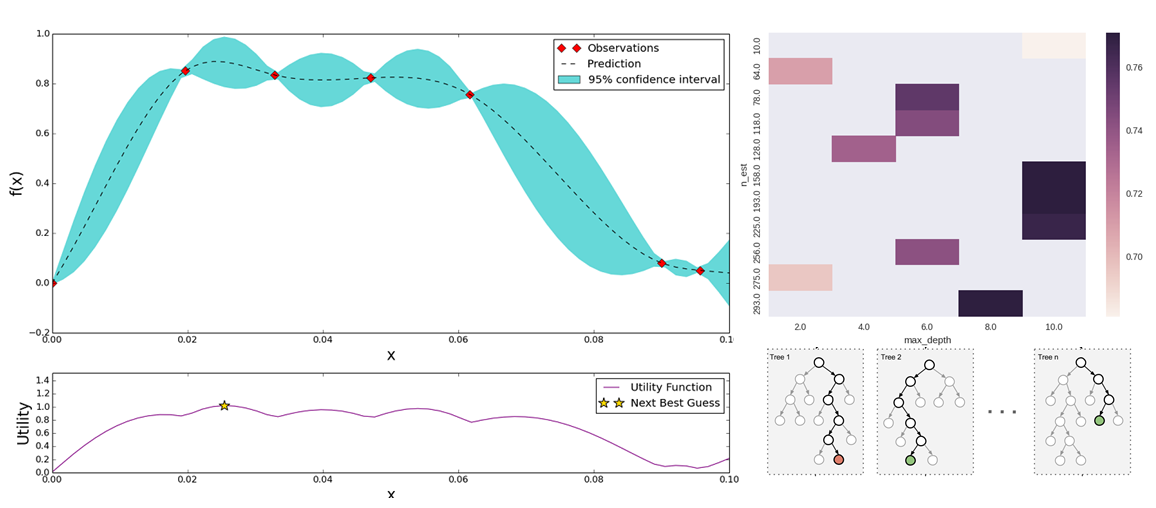
\includegraphics[width=0.95\textwidth, trim={10 10 10 10}]{figures/bayes_opt.png}
    \caption{Bayesian Optimization of SVM and Random Forest parameters}
    \label{fig:bayes_opt}
\end{figure}

Figure \ref{fig:bayes_opt} shows Baeysian optimization applied to SVM and Random Forest. F1 score was used as performance objective function for a classification task. The figure on the left shows Bayesian optimization of F1 score as a function of the gamma parameter of the SVM RBF kernel: $K(x,x^{\prime}) = \exp\{-\gamma ||x-x^{\prime}||^{2}\}$. We can see that after only 7 iterations we have discovered the gamma parameter that gives the maximum F1 score. The peak of EI utility function at the bottom tells us which experiment to perform next. The figure on the right shows Bayesian optimization of F1 score as a function of maximum depth and the number of estimators of a Random Forest classifier. From the heatmap, we can tell that the maximum F1 score is achieved for $158$ estimators with depth equal to $10$.    


\subsection{Active Learning}

The key idea behind active learning is that a machine learning algorithm can achieve greater accuracy with fewer training labels if it is allowed to choose the data from which it learns. Active learning is well motivated in many modern machine learning problems where unlabeled data may be abundant but labels are expensive to obtain. Active learning is sometimes called query learning or optimal experimental design because an active learner poses queries in the form of unlabelled data instances to be labeled by an oracle. In this way, the active learner seeks to achieve high accuracy using as few labeled instances as possible \cite{Settles2009}.\\

We focus on \textit{pool-based sampling} that assumes that there is a small set of labeled data $L$ and a large pool of unlabelled data $U$. Queries are selectively drawn from the pool according to an informativeness measure. Pool based methods rank the entire collection of unlabelled data to select the best query. Therefore, for very larget data-sets, stream-based sampling maybe more appropriate where the data is scanned sequentially and query decisions are evaluated individually.\\

\begin{figure}[tbhp]
    \centering
    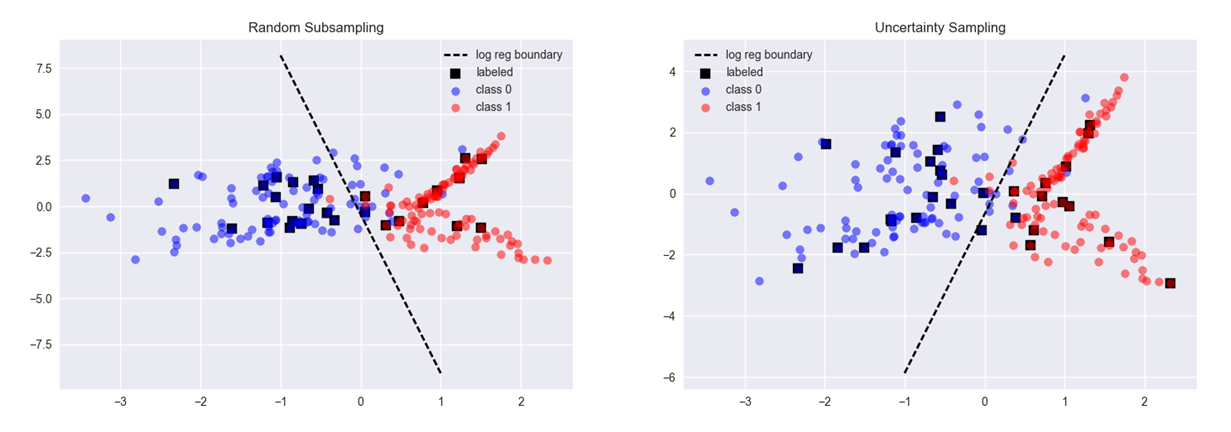
\includegraphics[width=0.95\textwidth, trim={10 10 10 10}]{figures/active_learning_logreg.png}
    \caption{Random Subsampling vs Uncertainty Sampling}
    \label{fig:al_logreg}
\end{figure}

Figure \ref{fig:al_logreg} shows an example of pool-based active learning based on binary classification of a synthetic dataset with two balanced classes using Logistic Regression (LR). On the left, we can see the LR decision boundary as a result of training on a randomly subsampled set of $30$ labels that achieves a classification accuracy of $90\%$ on held out data. On the right, we can see the LR decision boundary as a result of training on $30$ queries selected by uncertainty sampling based on entropy. Uncertainty sampling achieves a higher classification accuracy of $92.5\%$ on the held out set.   


\subsubsection{Query Strategies}

\textit{Uncertainty Sampling.} One of the simplest and most commonly used query framework is uncertainty sampling. In this framework, an active learner queries the label about which it is least certain. For example, in binary logistic regression, uncertainty sampling queries points near the boundary where the probability of being positive is close to $0.5$. For multi-class problems, uncertainty sampling can query points that are least confident:
\begin{equation}
    x_{LC}^{\ast} = \arg \max_x 1 - P_{\theta}(\hat{y}|x)
\end{equation}
where $\hat{y} \in \{1,...,K\}$ is the class label with the highest posterior probability under the model $\theta$. The criterion for the least confident strategy only considers information about the most probable label. We can use max margin sampling to preserve information about the remaining label distribution:
\begin{equation}
    x_{M}^{\ast} = \arg \min_x P_{\theta}(\hat{y}_1|x) - P_{\theta}(\hat{y}_2|x)
\end{equation}
where $\hat{y}_1$ and $\hat{y}_2$ are the first and second most probable class labels under the model, respectively. Intuitively, instances with large margins are easy to classify. Thus, points with small margins are ambiguous and knowing their labels would help the model to more effectively discriminate between them. However, for multi-class problems with very large label sets, the margin strategy still ignores much of the output distribution for the remaining classes. A more general uncertainty sampling strategy is based on entropy:
\begin{equation}
    x_{H}^{\ast} = \arg \max_x -\sum_i P_{\theta}(y_i|x)\log P_{\theta}(y_i|x)
\end{equation}
By learning labels that have highest entropy we can reduce label uncertainty. Uncertainty sampling also works for regression problems, in which case the learner queries the point with highest output variance in its prediction.\\

\textit{Query by Committee.} Another query selection framework is the Query By Committee (QBC) algorithm that involves maintaining a committee $C = \{\theta^{(1)},...,\theta^{(C)}\}$ of models which are all trained on the current labeled set $L$ but represent competing hypotheses. Each committee member is then allowed to vote on the labelings of query candidates and the most informative query is considered to be an instance about which they most disagree. The objective of QBC is to minimize a set of hypotheses that are consistent with the current labeled training data $L$. For measuring the level of disagreement two main approaches have been proposed \cite{Settles2009}: the vote entropy and KL divergence. The vote entropy is defined as follows:
\begin{equation}
    x_{VE}^{\ast} = \arg \max_x - \sum_i \frac{V(y_i)}{C} \log \frac{V(y_i)}{C}
\end{equation}
where $y_i \in \{1,...,K\}$ is the class label, $V(y_i)$ is the number of votes that a label received from the committee members and $C$ is the size of the committee. The KL divergence for QBC voting is defined as follows:
\begin{eqnarray}
    x_{KL}^{\ast} &=& \arg \max_x \frac{1}{C} \sum_{c=1}^{C} KL(P_{\theta^{(c)}}||P_C)\\
    KL(P_{\theta^{(c)}}||P_C) &=& \sum_i P_{\theta^{(c)}}(y_i|x) \log \frac{P_{\theta^{(c)}}(y_i|x)}{P_C(y_i|x)}\\
    P_C(y_i|x) &=& \frac{1}{C}\sum_{c=1}^{C}P_{\theta^{(c)}}(y_i|x)
\end{eqnarray}
where $\theta^{(c)}$ represents a member model of the committee and $P_C(y_i|x)$ is the consensus probability that $y_i$ is the correct label. The KL divergence metric considers the most informative query to be the one with the largest average difference between the label distributions of any one committee member and the consensus distribution.\\

\textit{Variance Reduction}. We can reduce the generalization error by minimizing output variance. Consider a regression problem for which the learning objective is to minimize the mean squared error. Let $\bar{\theta} = E[\hat{\theta}]$ be the expected value of the parameter estimate $\hat{\theta}$ and let $\theta^{\ast}$ be the ground truth, then
\begin{eqnarray}
   \mathrm{MSE} &=& E\bigg[(\hat{\theta} - \theta^{\ast})^{2} \bigg]  = E\bigg[\big[(\hat{\theta} - \bar{\theta})+(\bar{\theta} - \theta^{\ast}) \big]^{2} \bigg] \\
                &=& E\bigg[(\hat{\theta} - \bar{\theta})^{2} \bigg] + 2(\bar{\theta}-\theta^{\ast})E\bigg[\hat{\theta}-\bar{\theta}\bigg] + (\bar{\theta}-\theta^{\ast})^{2} \\
                &=& E\bigg[(\hat{\theta} - \bar{\theta})^{2} \bigg] +  (\bar{\theta}-\theta^{\ast})^{2} \\
                &=& \mathrm{VAR}[\hat{\theta}] + \mathrm{bias}^{2}(\hat{\theta})
\end{eqnarray}
This is called the \textbf{bias-variance tradeoff}. Thus, it is possible to achieve lower MSE with a biased estimator as long as it reduces the variance. A natural question is how low can the variance be? The answer is given by the Cramer-Rao lower bound that provides a lower bound on the variance of any unbiased estimator.
\begin{theorem}
(Cramer-Rao Lower Bound) Assuming $p(x|\theta)$ satisfies the regularity condition, the variance of any unbiased estimator $\hat{\theta}$ satisfies:
\begin{equation}
    \mathrm{VAR}(\hat{\theta}) \geq \frac{1}{-E\big[\frac{\partial^{2} \log p(x|\theta)}{\partial \theta^{2}} \big]} = \frac{1}{I(\theta)}
\end{equation}
where $I(\theta)$ is the Fisher information matrix. 
\end{theorem}
Thus, the Minimum Variance Unbiased (MVU) estimator achieves the minimum variance equal to the inverse of the Fisher information matrix. To minimize variance of parameter estimates, an active learner should select data that maximizes its Fisher information. For multi-variate models with $K$ parameters, Fisher information takes the form of a $K\times K$ matrix:
\begin{equation}
    [I(\theta)]_{ij} = -E \bigg[\frac{\partial^{2}\log p(x|\theta)}{\partial \theta_i \partial \theta_j} \bigg]
\end{equation}
As a result, there are several options for minimizing the inverse information matrix: A-optimality minimizes the trace: $Tr(I^{-1}(\theta))$, D-optimality minimizes the determinant: $|I^{-1}(\theta)|$ and E-optimality minimizes the maximum eigenvalue: $\lambda_{max}[I^{-1}(\theta)]$.\\

However, there are some computational disadvantages to the variance reduction methods. Estimating output variance requires inverting a $K\times K$ matrix for each unlabeled instance, resulting in a time complexity of $\mathcal{O}(UK^{3})$, where $U$ is the size of the query pool. As a result variance reduction methods are empirically slower than simpler query strategies like uncertainty sampling.\\  

Active learning and \textit{semi-supervised learning} both try to make the most of unlabeled data. For example, a basic semi-supervised technique is self-training in which the learner is first trained with a small amount of labeled data and then used to classify the unlabeled data. The most confident unlabeled instances together with their predicted labels are added to the training set and the process repeats.\\ 

\begin{figure}[tbhp]
    \centering
    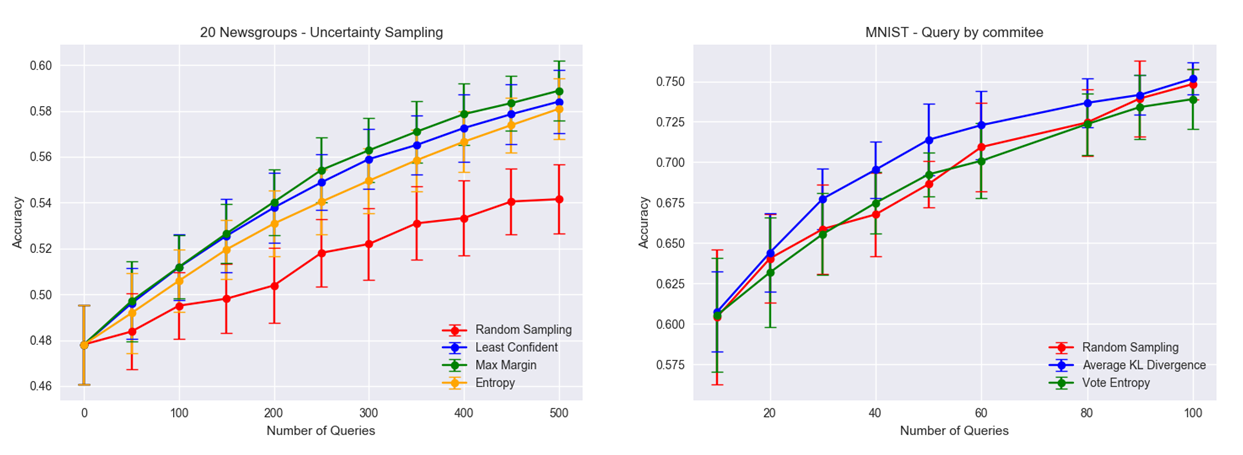
\includegraphics[width=0.95\textwidth, trim={10 10 10 10}]{figures/active_learning_merged.png}
    \caption{Active Learning: Uncertainty Sampling and Query By Committee.}
    \label{fig:al_merged}
\end{figure}

Figure \ref{fig:al_merged} compares $3$ uncertainty sampling techniques: least confident, max margin and entropy with a random subsampling baseline on 20 newsgroups dataset classified with Logistic Regression. All three methods achieve higher accuracy in comparison to baseline that highlights the benefit of active learning. On the right, we can see the performance of Query By Committee strategy applied to MNIST dataset. The committee consists of $5$ instances of Logistic Regression. Two methods are compared against the random subsampling baseline: vote entropy and average KL divergence. We can see that average KL divergence achieves highest classification accuracy. All experiments were repeated $10$ times.  











